
\DIFaddbegin 

\clearpage
\subsection{\DIFadd{The Metal merchant}}
\label{sec:appendix:moj:metal}

\DIFadd{Viking metal smiths were called jarnsmithir. They made brooches, rings, and buckles out of iron, bronze, silver, pewter and gold.
}

\begin{display}{The metal stall}
	\label{fig:appendix:moj:places:metal:stall}
	\DIFadd{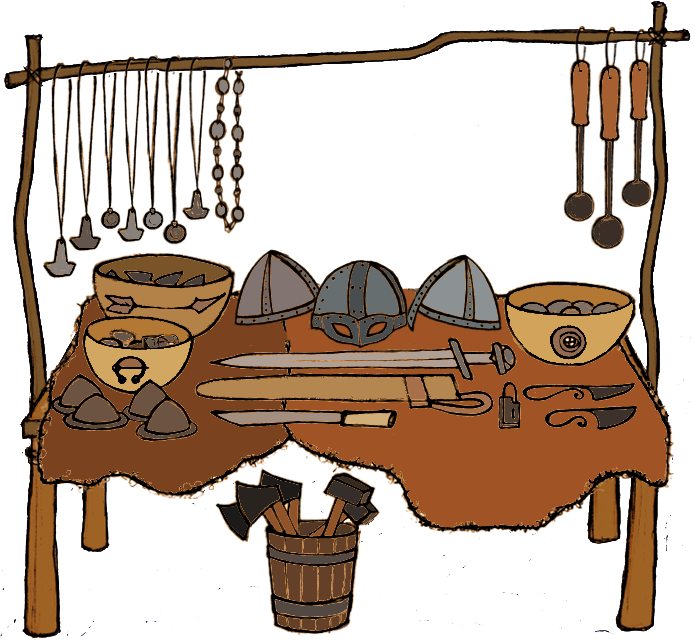
\includegraphics[width=0.65\columnwidth]{img/Jorvik/places/metal stall}
}\end{display}

\begin{display}{The metal stall with a background and a merchant}
	\label{fig:appendix:moj:places:metal}
	\DIFadd{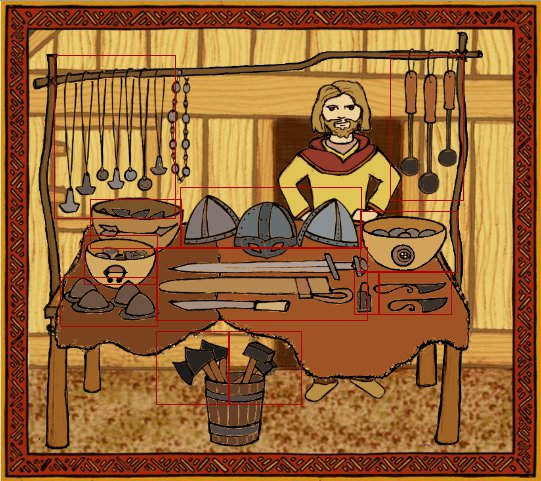
\includegraphics[width=0.65\columnwidth]{img/Jorvik/places/metal}
}\end{display}
\clearpage


\begin{table}[ht!]
	\centering
	\begin{tabular}{ p{3cm} c }\toprule
		\textbf{\DIFaddFL{Name:}} & \multirow{5}{*}{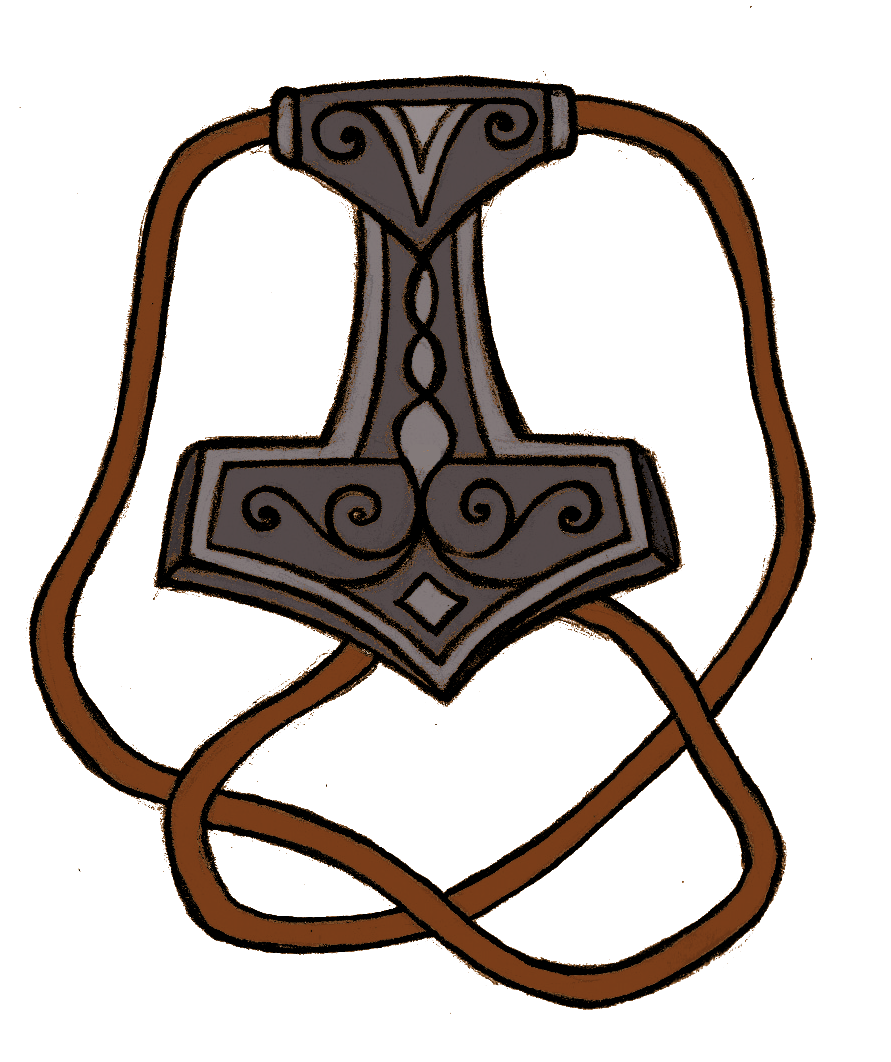
\includegraphics[height=30mm]{img/Jorvik/objects/metal/thors hammer}}\\
		\DIFaddFL{Thor'S Hammer }& \\ 
		\textbf{\DIFaddFL{Price:}} & \\
		\DIFaddFL{8.82 silver }& \\ 
		\textbf{\DIFaddFL{Description:}} & \\
		\multicolumn{2}{p{12cm}}{Thor, the Norse God of Thunder, had a magic hammer called Mjolnir. Vikings would wear pendants in the shape of Mjolnir as tribute to Thor. It could have come into fashion in defiance of the square amulets worn by newly converted Christians.}\\
		\bottomrule
	\end{tabular}
\end{table}

\begin{table}[ht!]
	\centering
	\begin{tabular}{ p{3cm} c }\toprule
		\textbf{\DIFaddFL{Name:}} & \multirow{5}{*}{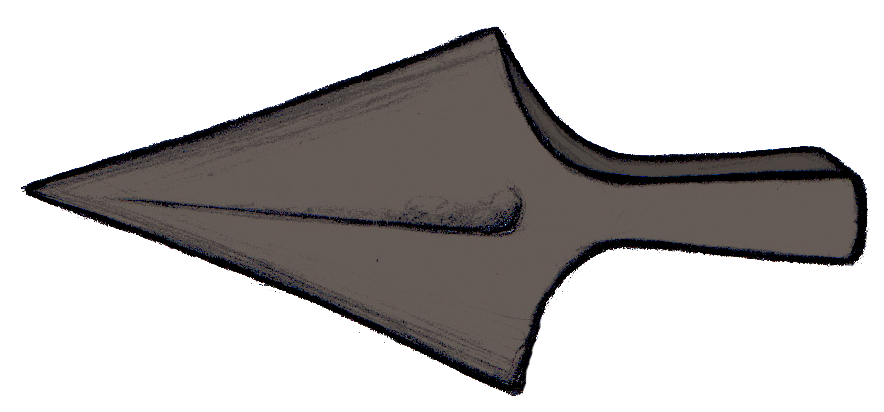
\includegraphics[height=30mm]{img/Jorvik/objects/metal/arrow head}}\\
		\DIFaddFL{Arrow Head }& \\ 
		\textbf{\DIFaddFL{Price:}} & \\
		\DIFaddFL{1.32 silver }& \\ 
		\textbf{\DIFaddFL{Description:}} & \\
		\multicolumn{2}{p{12cm}}{Vikings tended to use bows and arrows for hunting rather than fighting in battle. In England, the Vikings would have hunted wild boar, deer and hare.}\\
		\bottomrule
	\end{tabular}
\end{table}

\begin{table}[ht!]
	\centering
	\begin{tabular}{ p{3cm} c }\toprule
		\textbf{\DIFaddFL{Name:}} & \multirow{5}{*}{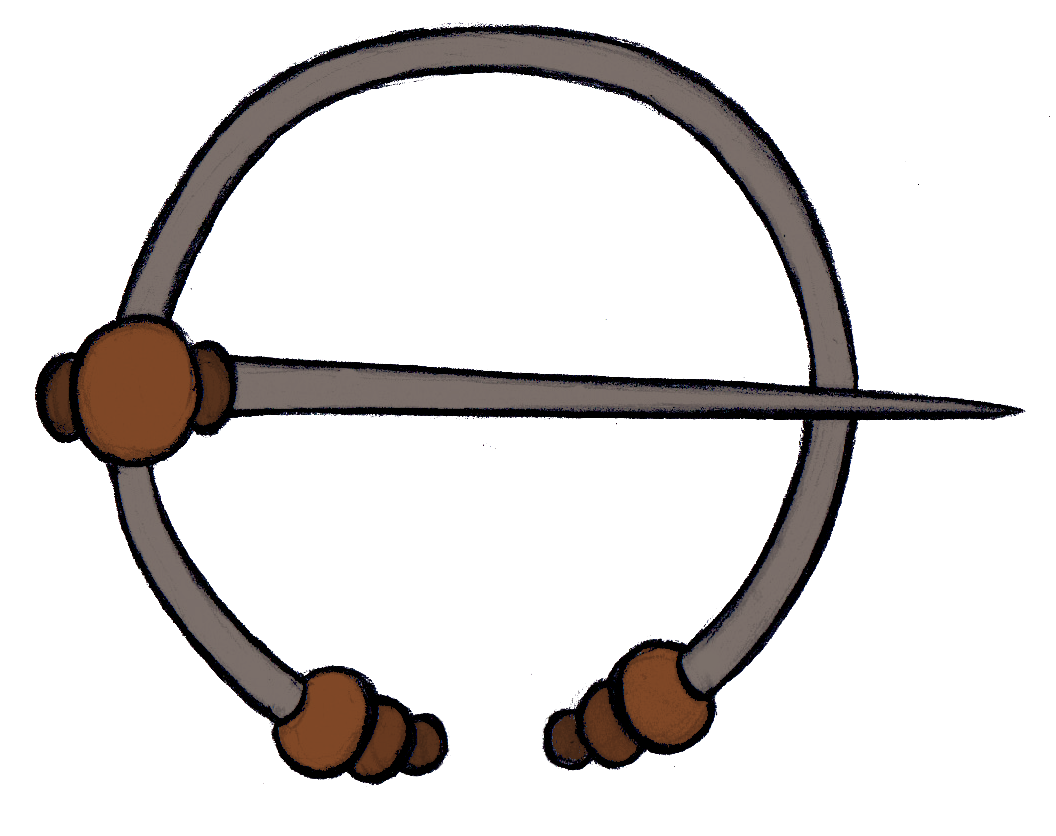
\includegraphics[height=30mm]{img/Jorvik/objects/metal/thistle brooch}}\\
		\DIFaddFL{Thistle Brooch }& \\ 
		\textbf{\DIFaddFL{Price:}} & \\
		\DIFaddFL{5.29 silver }& \\ 
		\textbf{\DIFaddFL{Description:}} & \\
		\multicolumn{2}{p{12cm}}{The thistle brooch came from Ireland in the 9th century and it was a popular design with the Vikings. Under Viking rule Dublin in Ireland was called Dyflin and, like Jorvik, was a big trading city.}\\
		\bottomrule
	\end{tabular}
\end{table}

\begin{table}[ht!]
	\centering
	\begin{tabular}{ p{3cm} c }\toprule
		\textbf{\DIFaddFL{Name:}} & \multirow{5}{*}{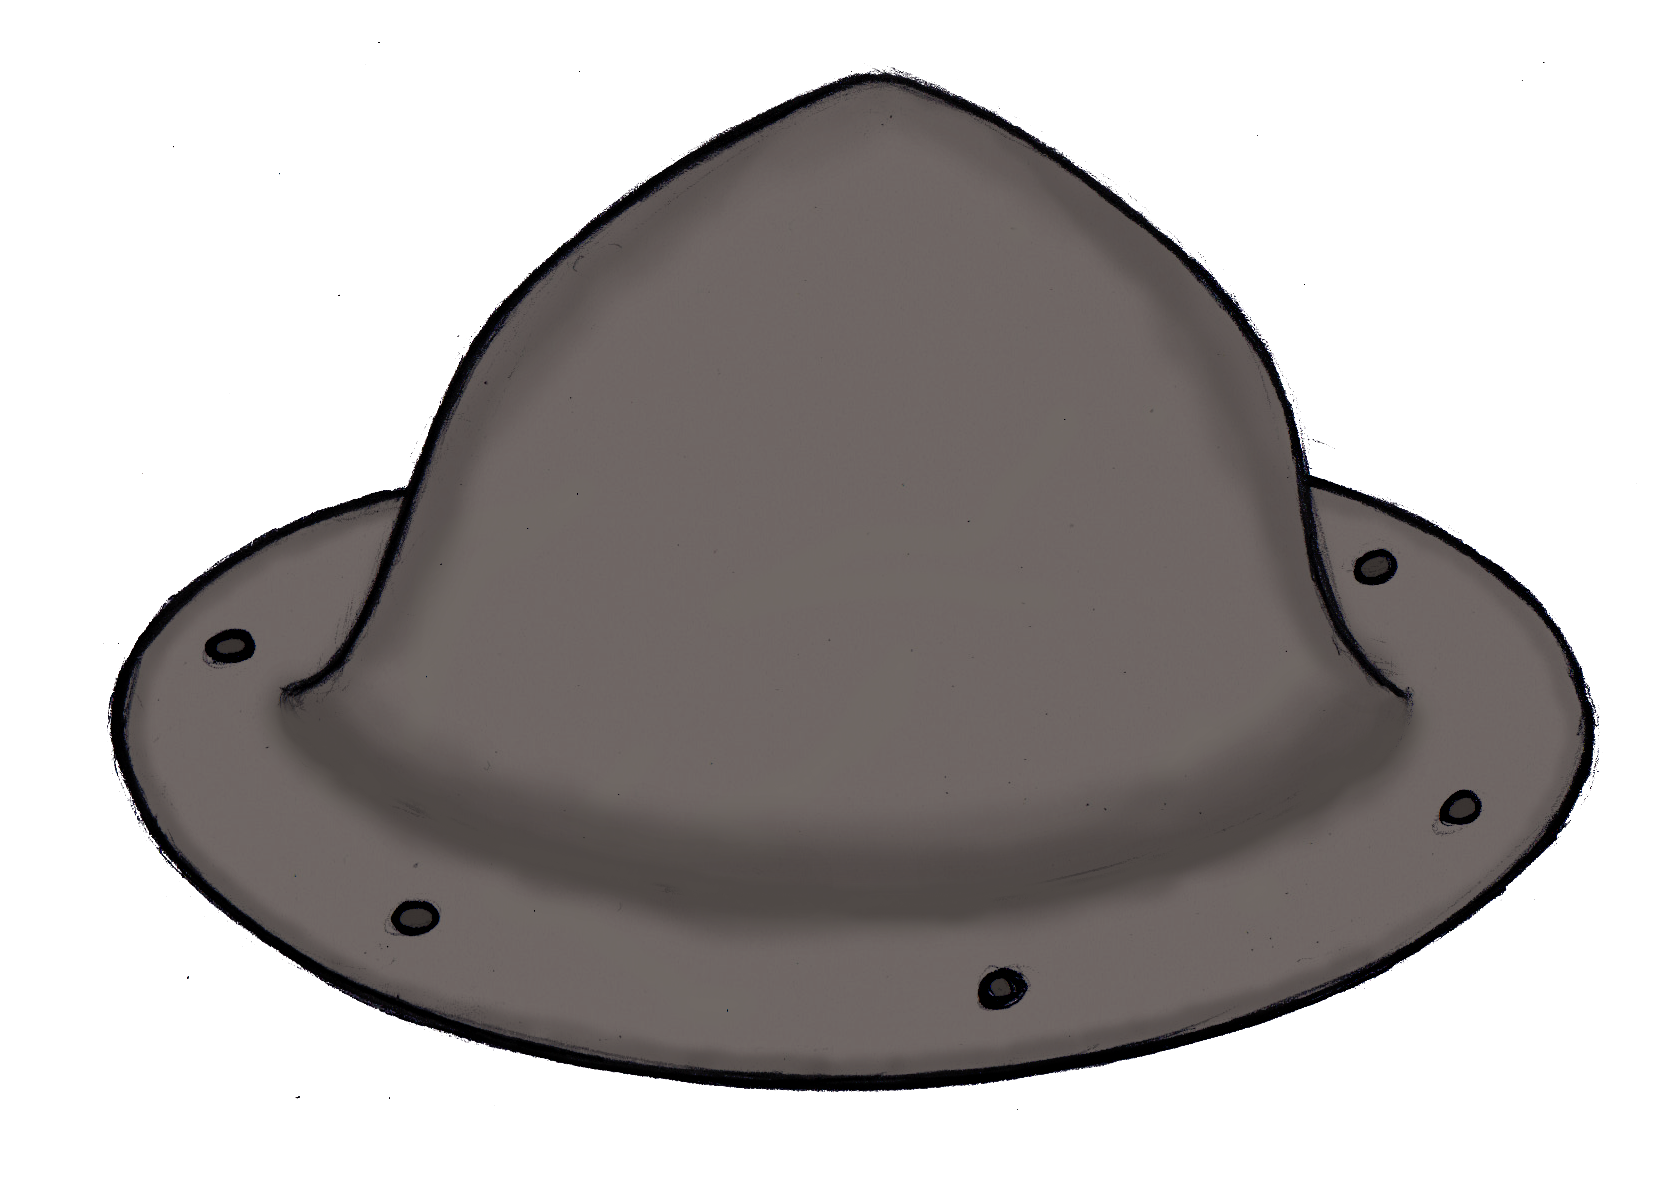
\includegraphics[height=30mm]{img/Jorvik/objects/metal/boss}}\\
		\DIFaddFL{Boss }& \\ 
		\textbf{\DIFaddFL{Price:}} & \\
		\DIFaddFL{3.53 silver }& \\ 
		\textbf{\DIFaddFL{Description:}} & \\
		\multicolumn{2}{p{12cm}}{A boss is the metal dome in the centre of a Viking shield. It strengthens the shield so that it won't break on impact with an axe or sword. It also protects the hand of the warrior who wields it.}\\
		\bottomrule
	\end{tabular}
\end{table}

\begin{table}[ht!]
	\centering
	\begin{tabular}{ p{3cm} c }\toprule
		\textbf{\DIFaddFL{Name:}} & \multirow{5}{*}{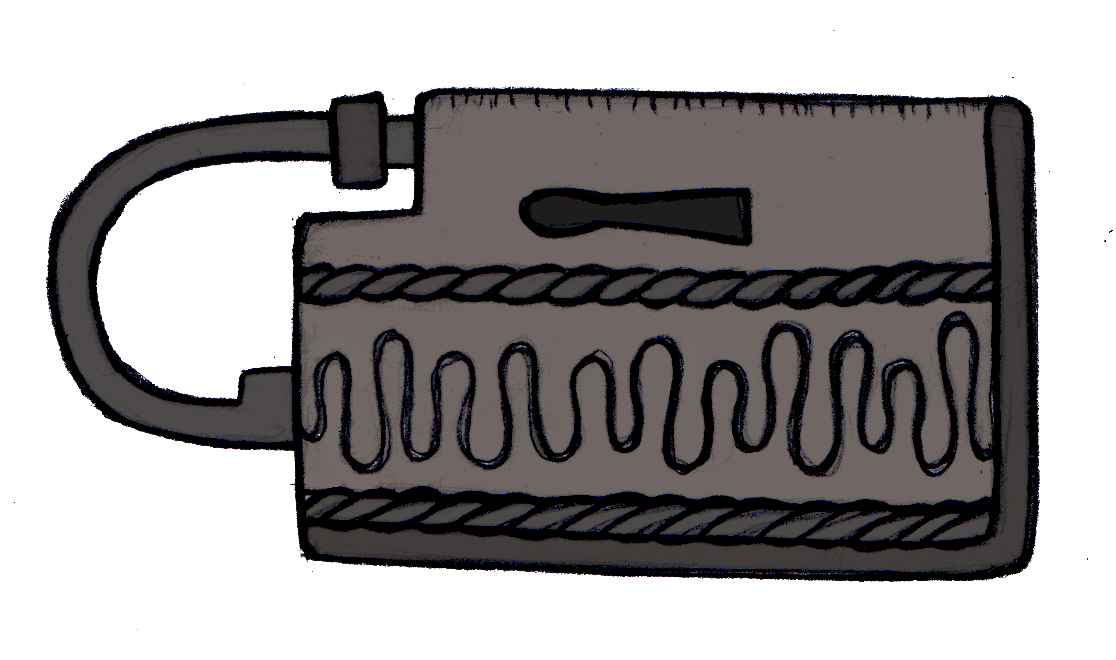
\includegraphics[height=30mm]{img/Jorvik/objects/metal/padlock}}\\
		\DIFaddFL{Padlock }& \\ 
		\textbf{\DIFaddFL{Price:}} & \\
		\DIFaddFL{3.09 silver }& \\ 
		\textbf{\DIFaddFL{Description:}} & \\
		\multicolumn{2}{p{12cm}}{With such a difficult lifestyle, each Viking family had to protect themselves and their home. Padlocks could secure doors and chests. It was the woman of the household who would carry keys to the home.}\\
		\bottomrule
	\end{tabular}
\end{table}

\begin{table}[ht!]
	\centering
	\begin{tabular}{ p{3cm} c }\toprule
		\textbf{\DIFaddFL{Name:}} & \multirow{5}{*}{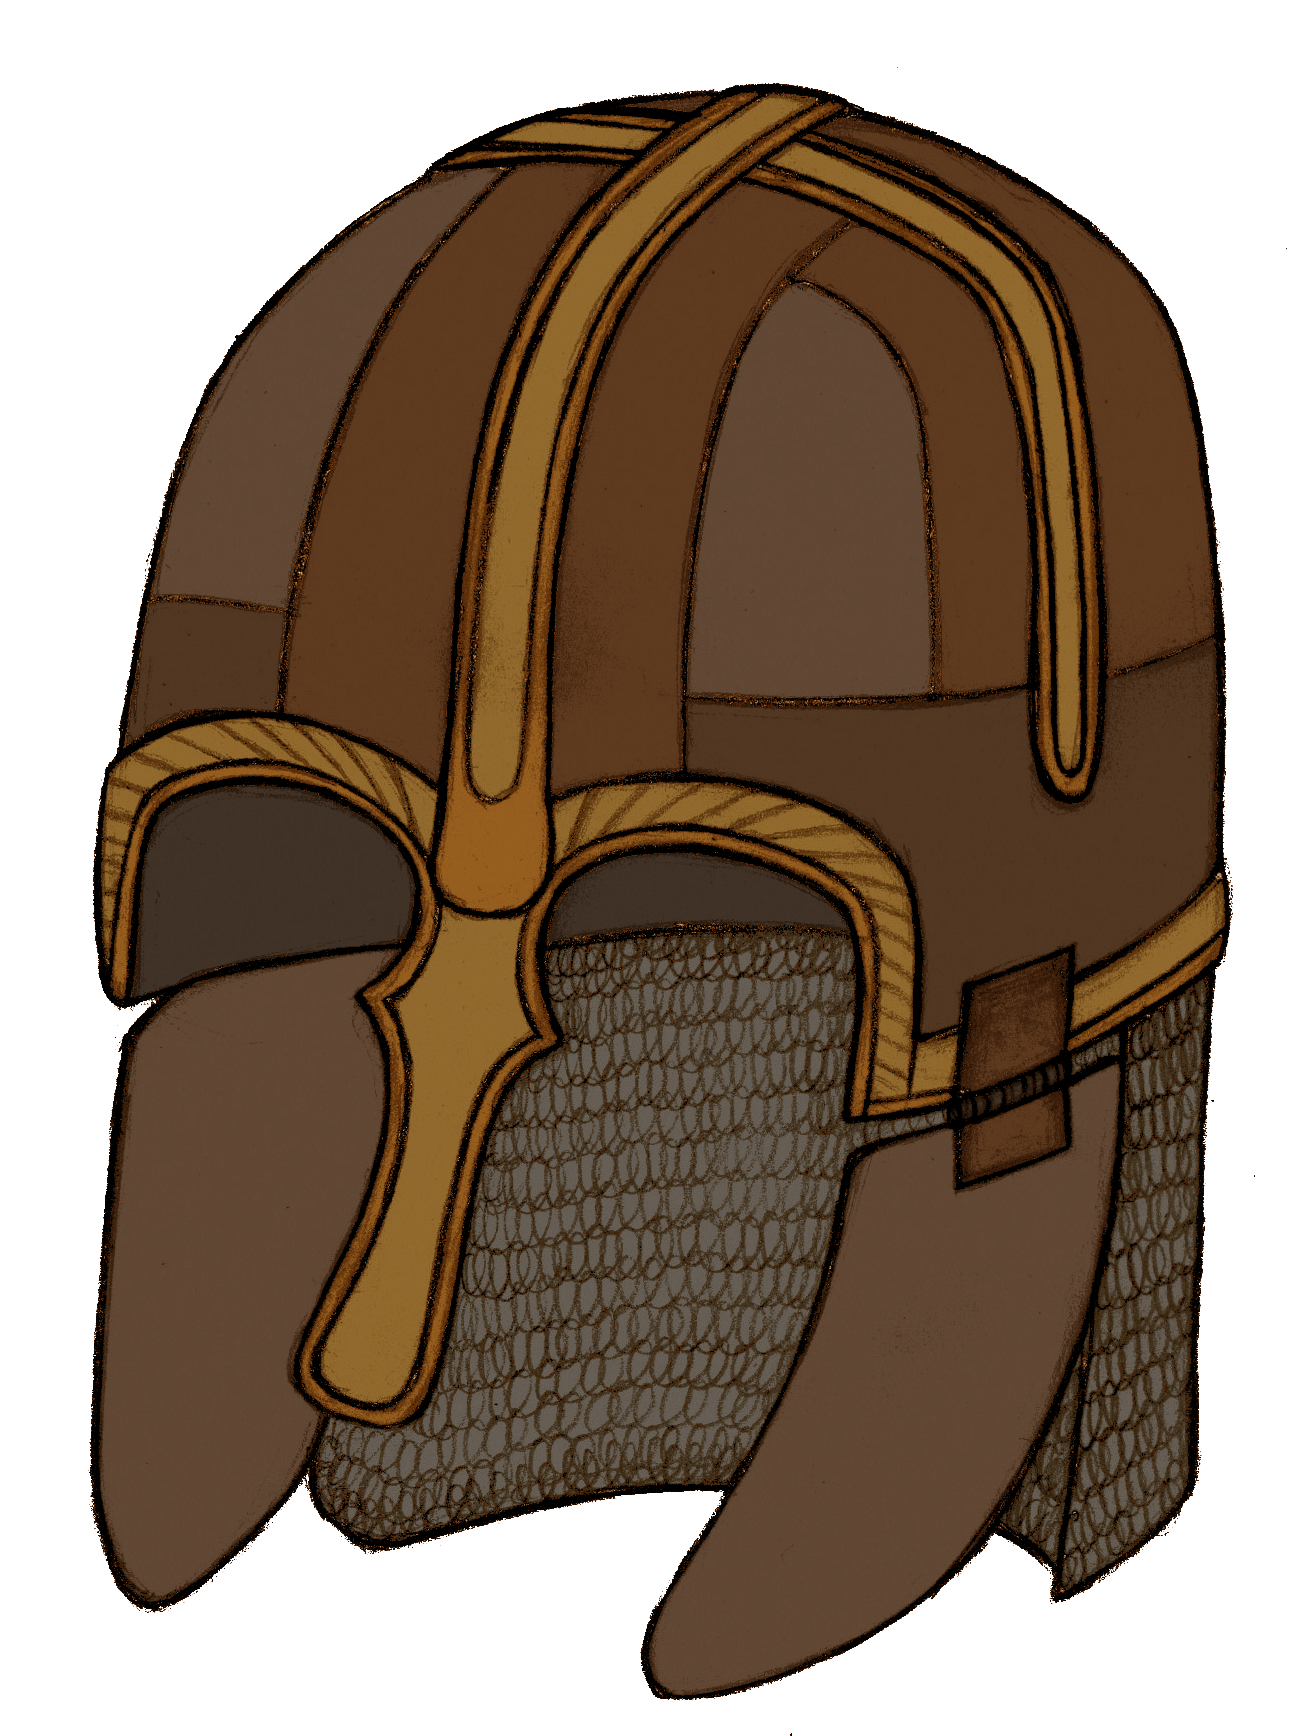
\includegraphics[height=30mm]{img/Jorvik/objects/metal/helmet}}\\
		\DIFaddFL{Helmet }& \\ 
		\textbf{\DIFaddFL{Price:}} & \\
		\DIFaddFL{23.38 silver }& \\ 
		\textbf{\DIFaddFL{Description:}} & \\
		\multicolumn{2}{p{12cm}}{Viking helmets did not have horns on them, as many people think. Because they were made of metal, they were very expensive and passed down through the generations.}\\
		\bottomrule
	\end{tabular}
\end{table}

\begin{table}[ht!]
	\centering
	\begin{tabular}{ p{3cm} c }\toprule
		\textbf{\DIFaddFL{Name:}} & \multirow{5}{*}{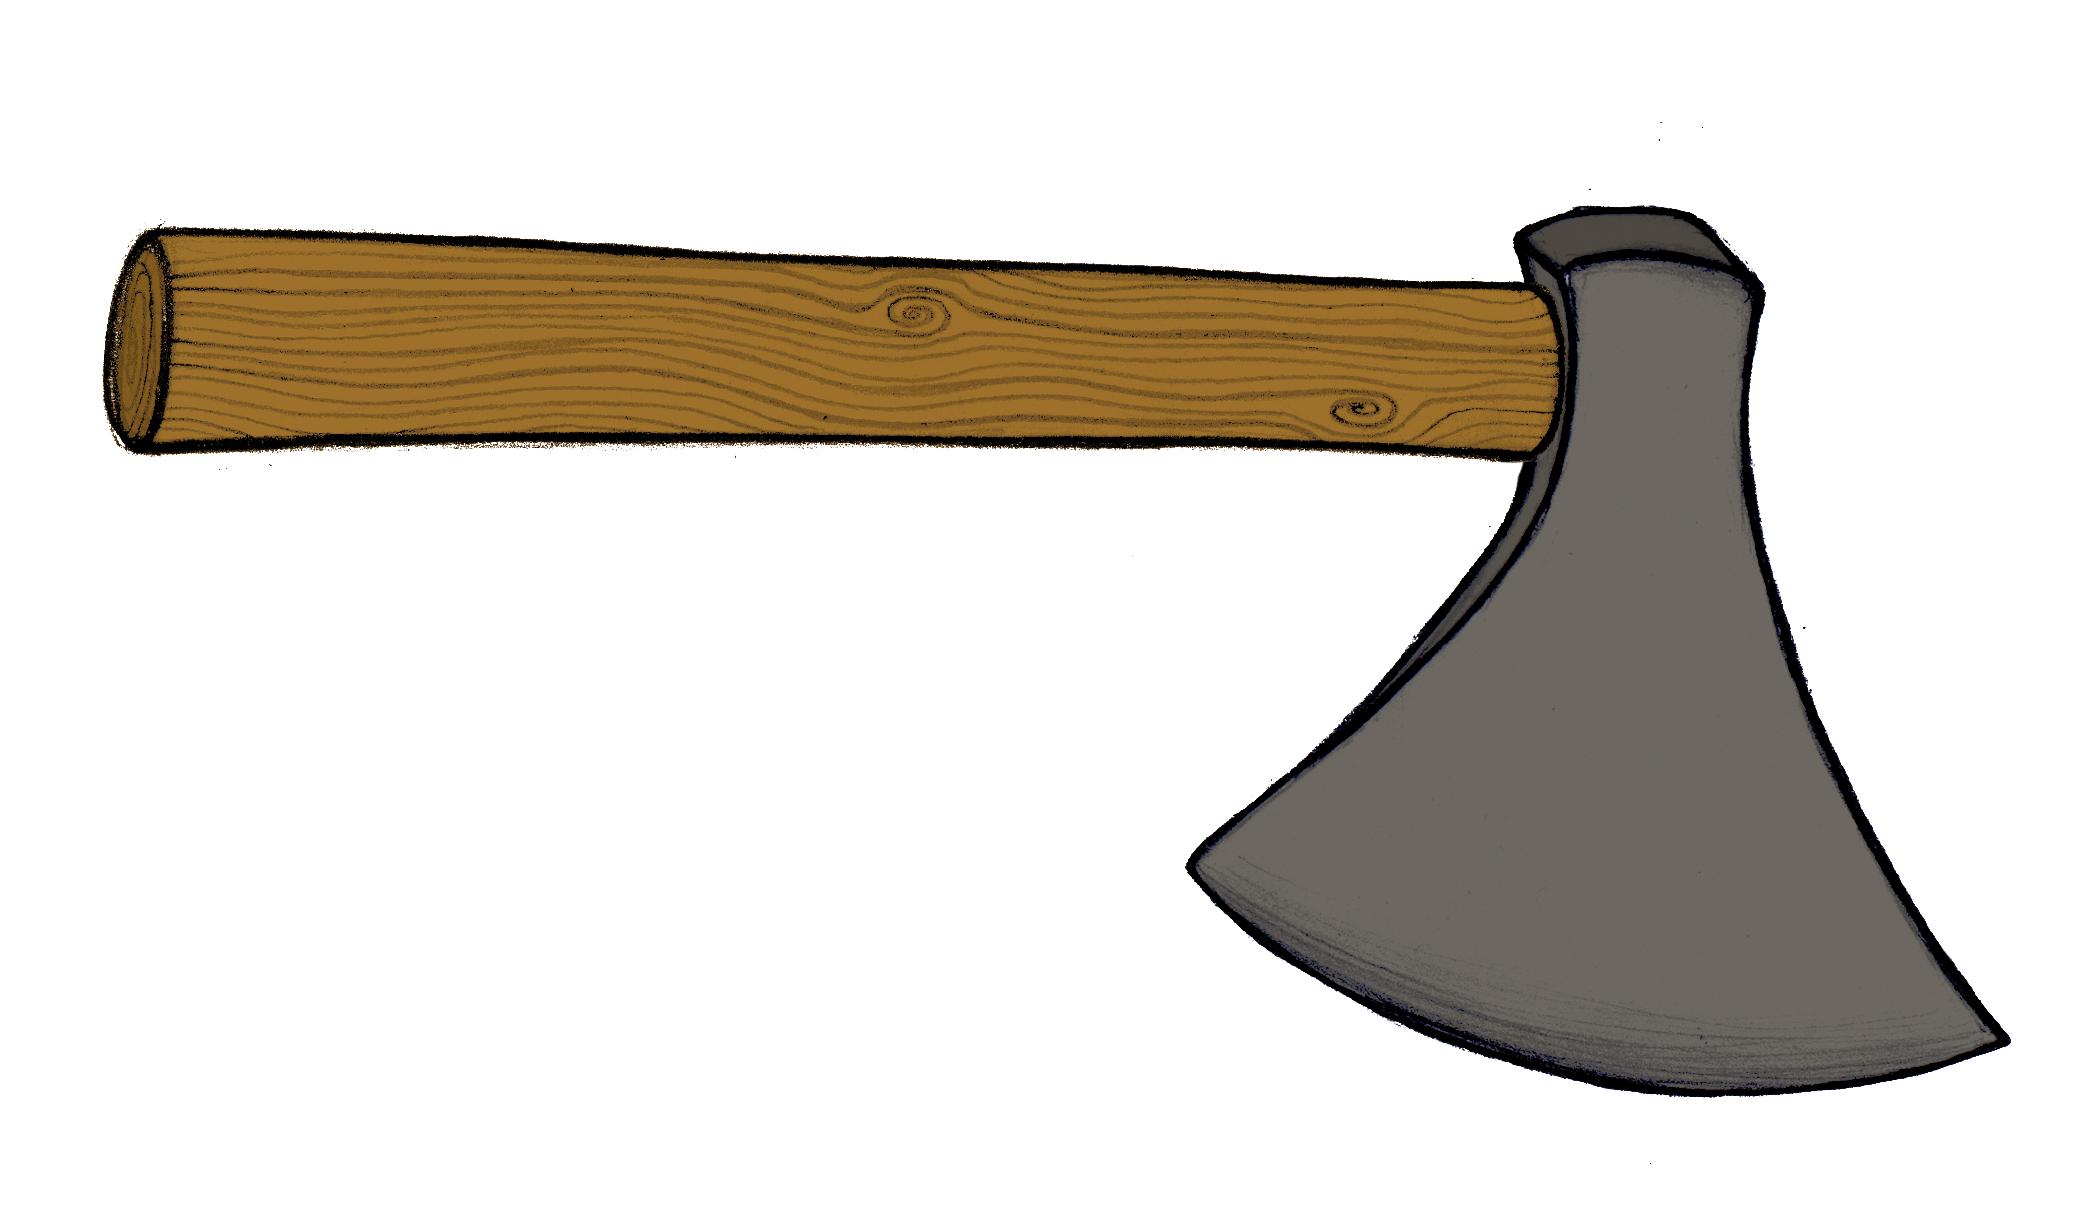
\includegraphics[height=30mm]{img/Jorvik/objects/metal/axe}}\\
		\DIFaddFL{Axe }& \\ 
		\textbf{\DIFaddFL{Price:}} & \\
		\DIFaddFL{13.23 silver }& \\ 
		\textbf{\DIFaddFL{Description:}} & \\
		\multicolumn{2}{p{12cm}}{An axe was a Viking's most useful tool. It could be used to chop firewood and other materials and it could also be used in battle.}\\
		\bottomrule
	\end{tabular}
\end{table}

\begin{table}[ht!]
	\centering
	\begin{tabular}{ p{3cm} c }\toprule
		\textbf{\DIFaddFL{Name:}} & \multirow{5}{*}{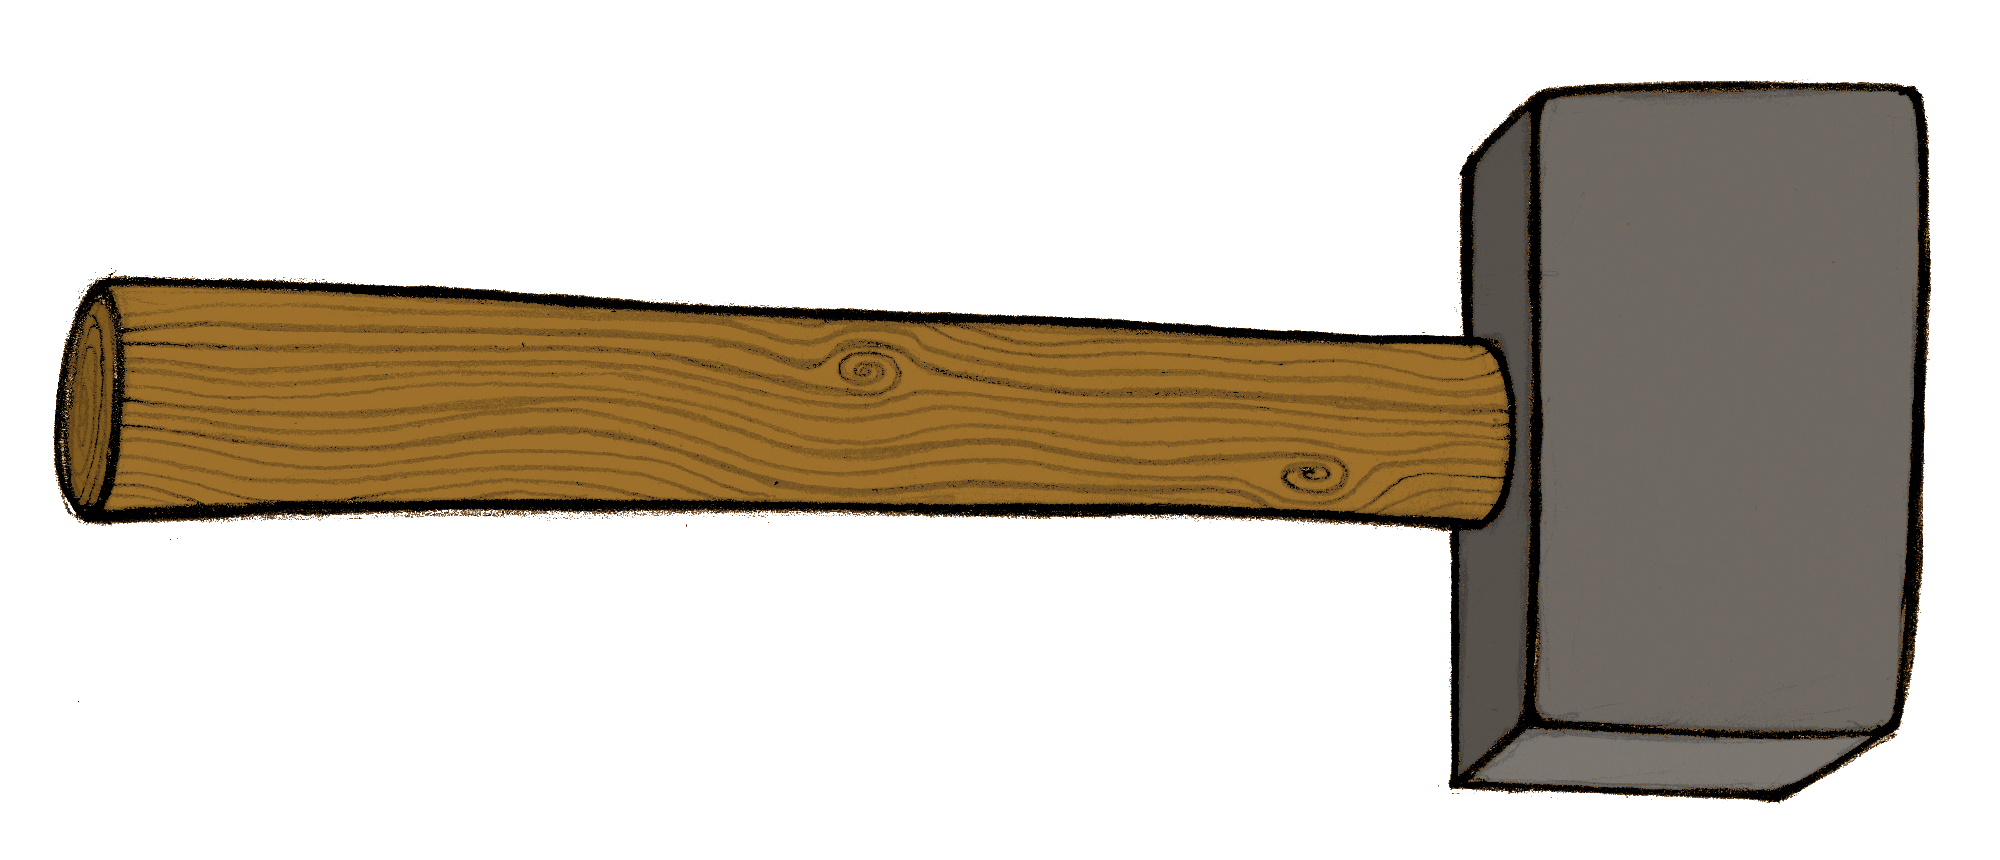
\includegraphics[width=70mm]{img/Jorvik/objects/metal/hammer}}\\
		\DIFaddFL{Hammer }& \\ 
		\textbf{\DIFaddFL{Price:}} & \\
		\DIFaddFL{8.82 silver }& \\ 
		\textbf{\DIFaddFL{Description:}} & \\
		\multicolumn{2}{p{12cm}}{Hammers were used to build houses and by blacksmiths in metal-working. York Archaeological Trust found a Viking house that had been built with two storeys – one on ground level and one below. The cellar was built using wood from the hull of a Viking ship!}\\
		\bottomrule
	\end{tabular}
\end{table}

\begin{table}[ht!]
	\centering
	\begin{tabular}{ p{3cm} c }\toprule
		\textbf{\DIFaddFL{Name:}} & \multirow{5}{*}{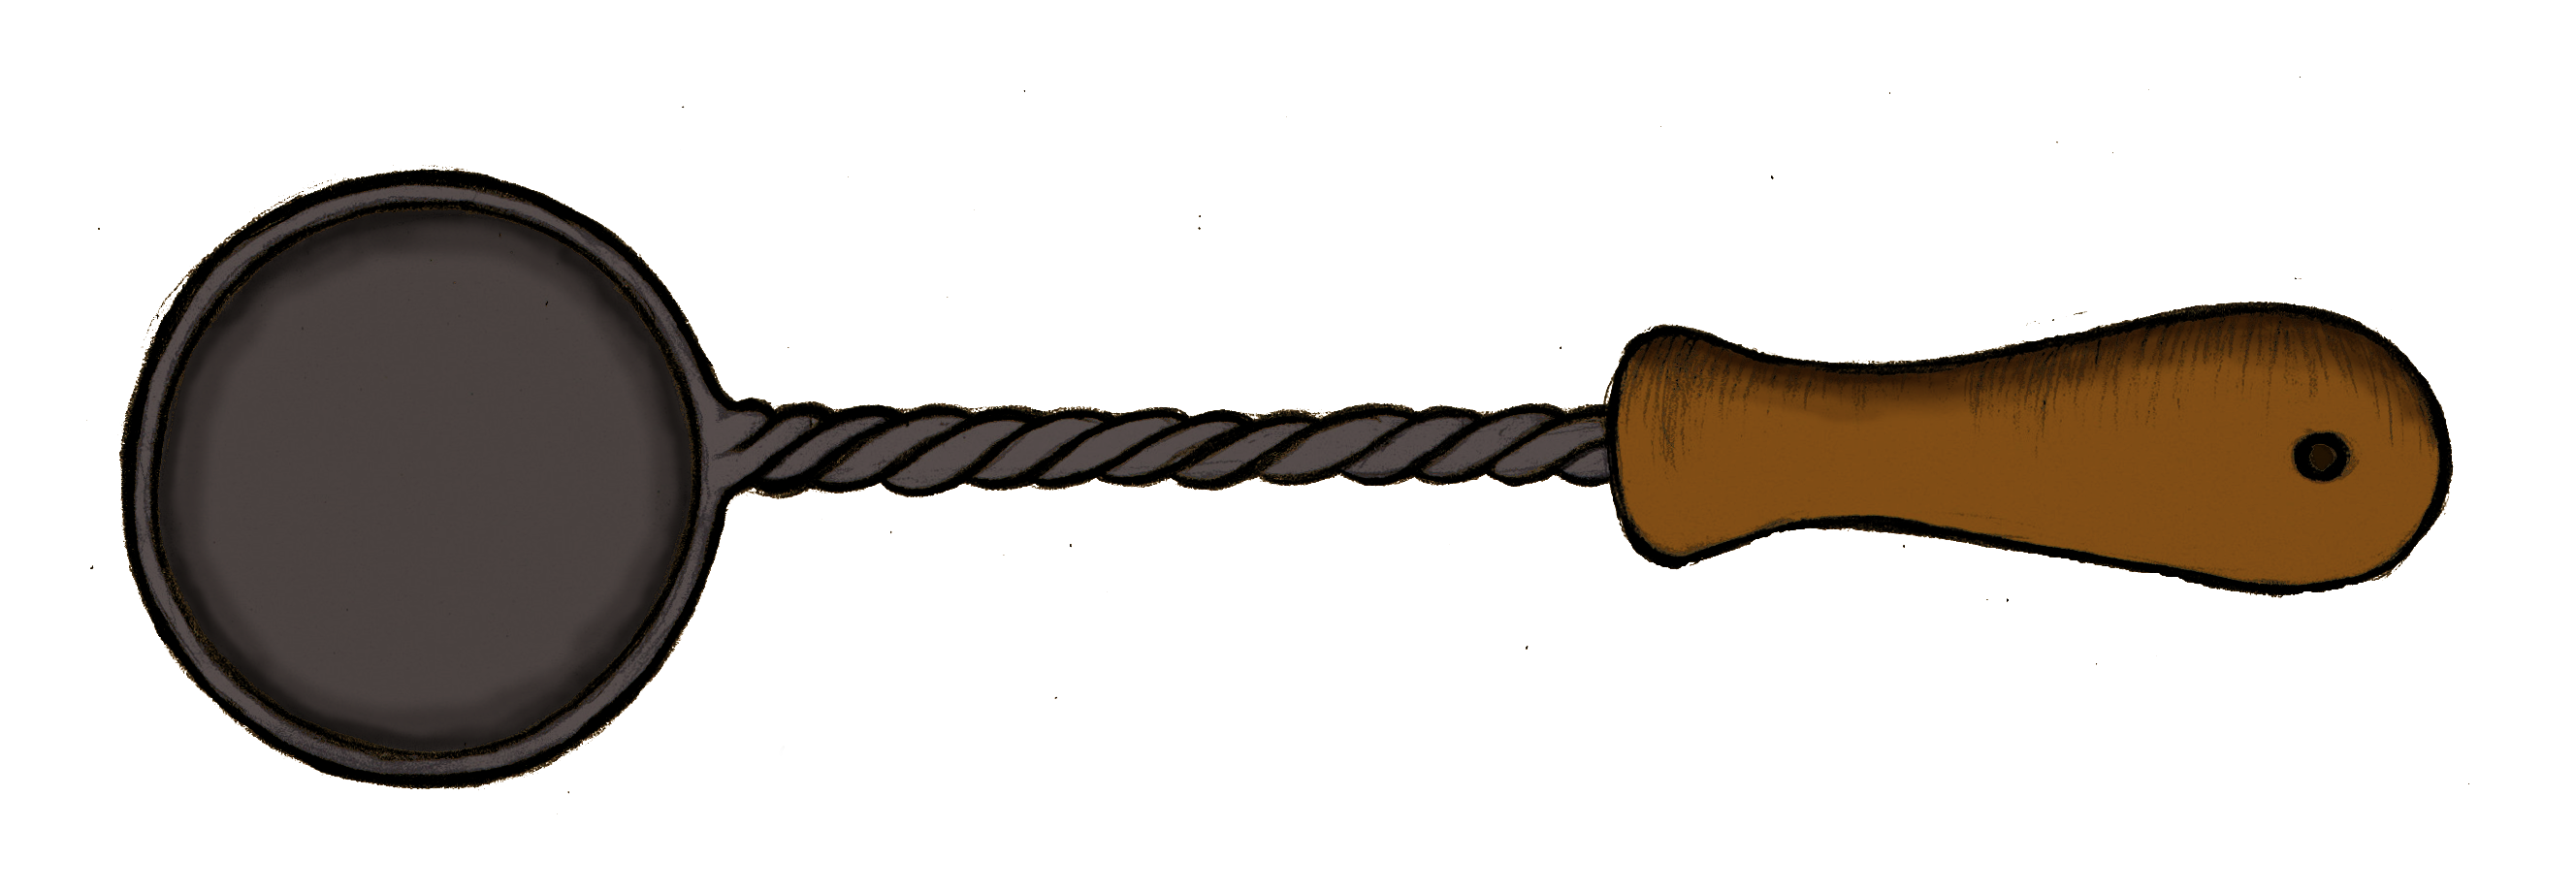
\includegraphics[width=70mm]{img/Jorvik/objects/metal/ladle}}\\
		\DIFaddFL{Ladle }& \\ 
		\textbf{\DIFaddFL{Price:}} & \\
		\DIFaddFL{5.73 silver }& \\ 
		\textbf{\DIFaddFL{Description:}} & \\
		\multicolumn{2}{p{12cm}}{Ladles were used to serve drinks into cups for everyday use and drinking horns for cold alcoholic drinks at feasts. A Viking woman was found buried with a ladle and a bucket in Skei, Norway.}\\
		\bottomrule
	\end{tabular}
\end{table}

\begin{table}[ht!]
	\centering
	\begin{tabular}{ p{3cm} c }\toprule
		\textbf{\DIFaddFL{Name:}} & \multirow{5}{*}{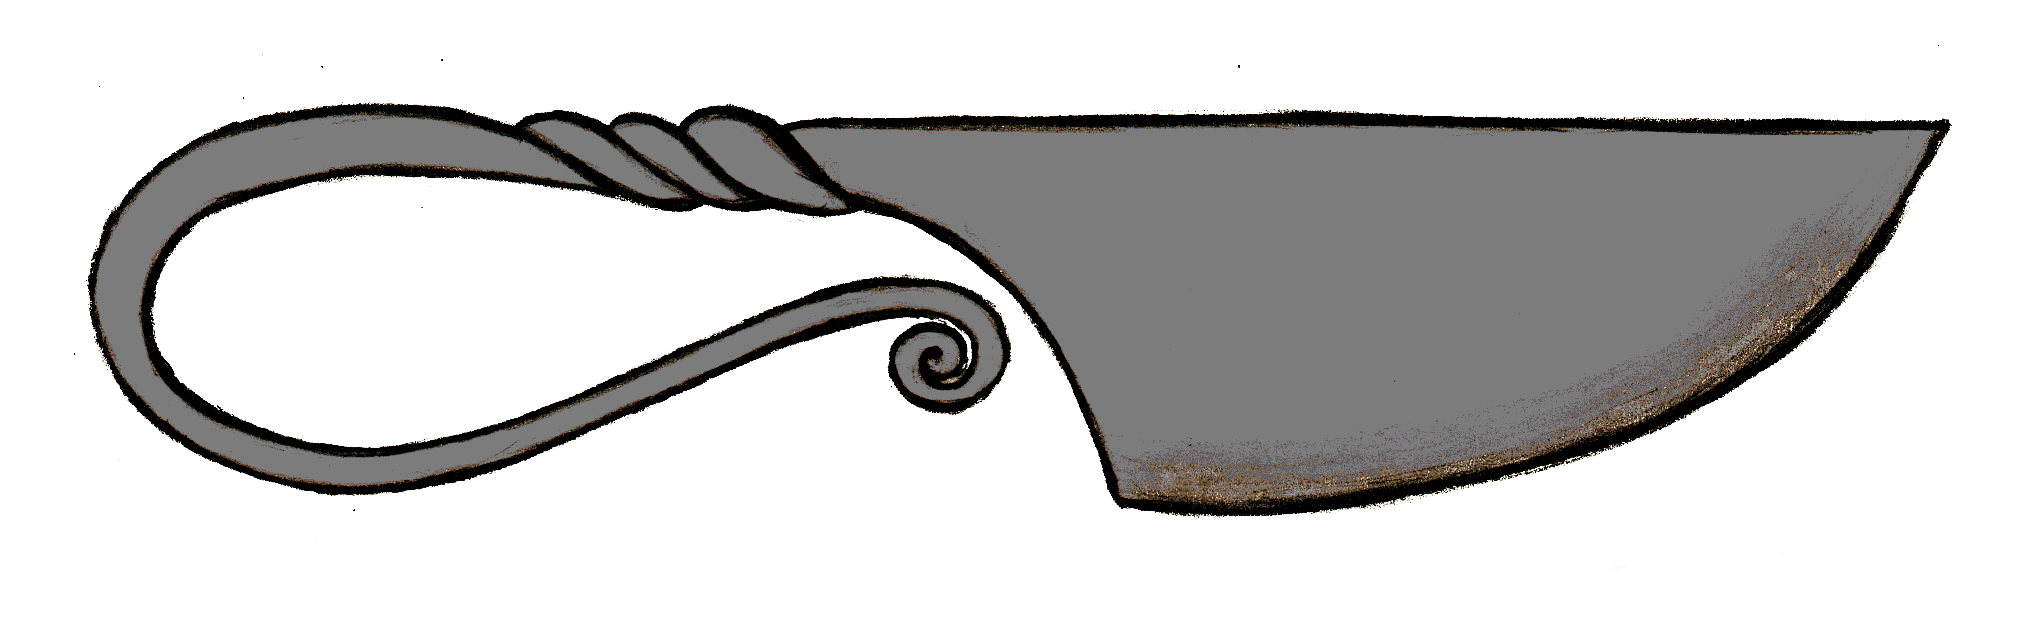
\includegraphics[width=70mm]{img/Jorvik/objects/metal/small knife}}\\
		\DIFaddFL{Small Knife }& \\ 
		\textbf{\DIFaddFL{Price:}} & \\
		\DIFaddFL{1.32silver }& \\ 
		\textbf{\DIFaddFL{Description:}} & \\
		\multicolumn{2}{p{12cm}}{A knife could be used for a wide range of uses including cutting vegetables, meat, thread and cloth. It was an essential tool to have in a Viking home.}\\
		\bottomrule
	\end{tabular}
\end{table}

\begin{table}[ht!]
	\centering
	\begin{tabular}{ p{3cm} c }\toprule
		\textbf{\DIFaddFL{Name:}} & \multirow{5}{*}{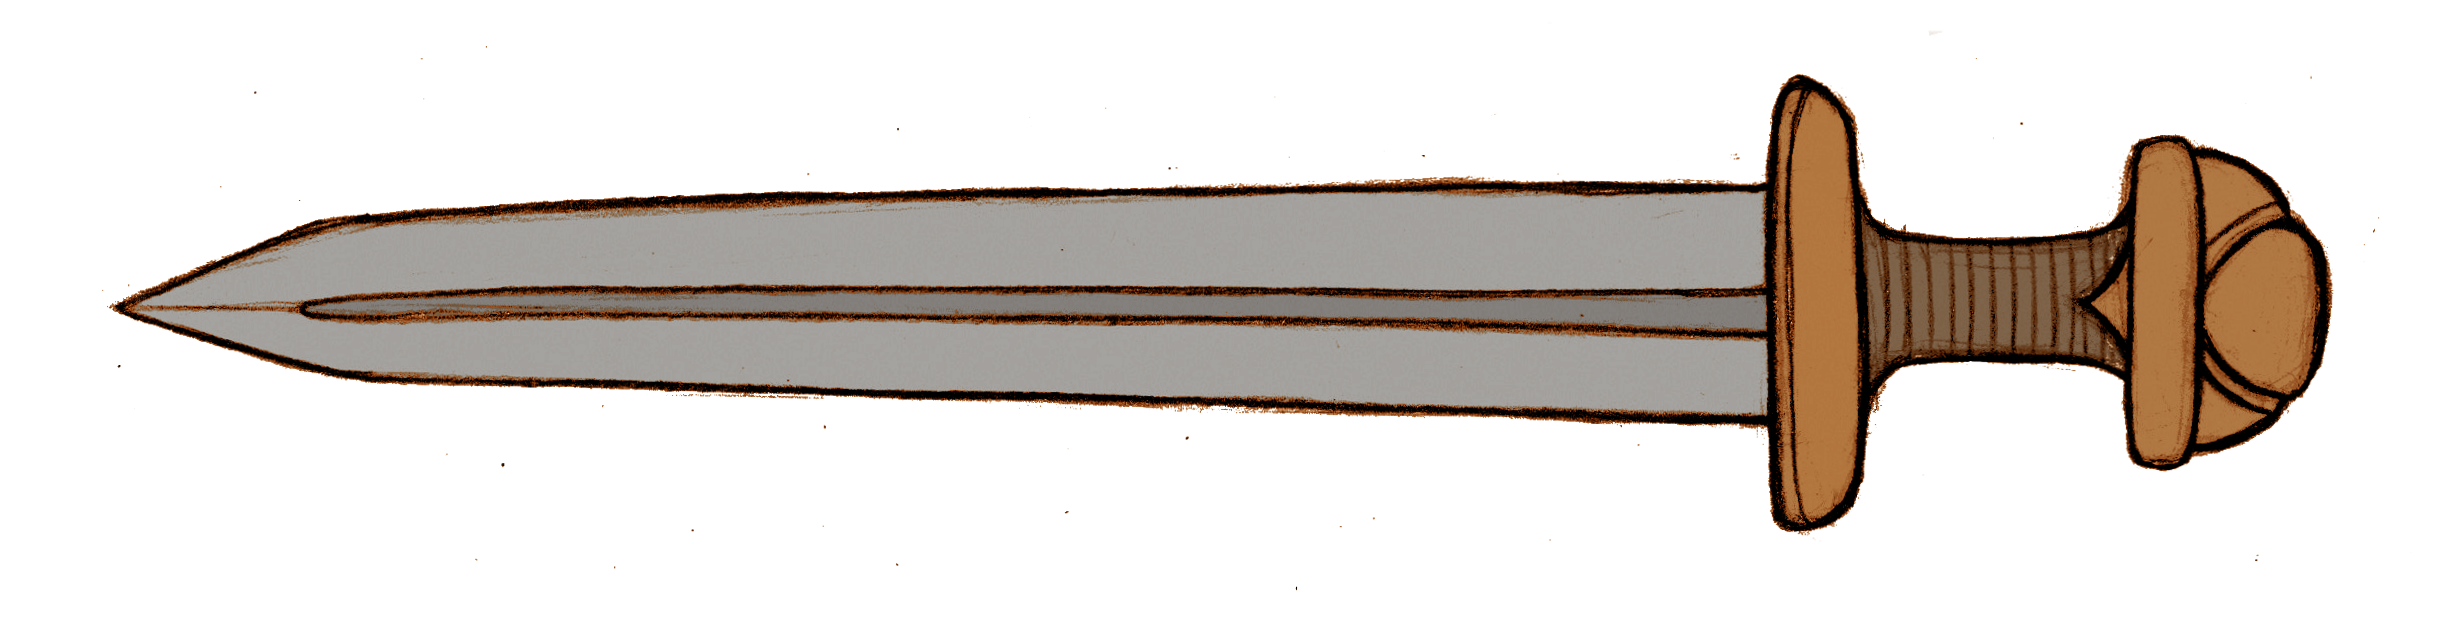
\includegraphics[width=70mm]{img/Jorvik/objects/metal/sword}}\\
		\DIFaddFL{Sword }& \\ 
		\textbf{\DIFaddFL{Price:}} & \\
		\DIFaddFL{820.40 silver }& \\ 
		\textbf{\DIFaddFL{Description:}} & \\
		\multicolumn{2}{p{12cm}}{A sword was a very expensive weapon and would be kept in the family and passed down from fathers to sons.}\\
		\bottomrule
	\end{tabular}
\end{table}

\begin{table}[ht!]
	\centering
	\begin{tabular}{ p{3cm} c }\toprule
		\textbf{\DIFaddFL{Name:}} & \multirow{5}{*}{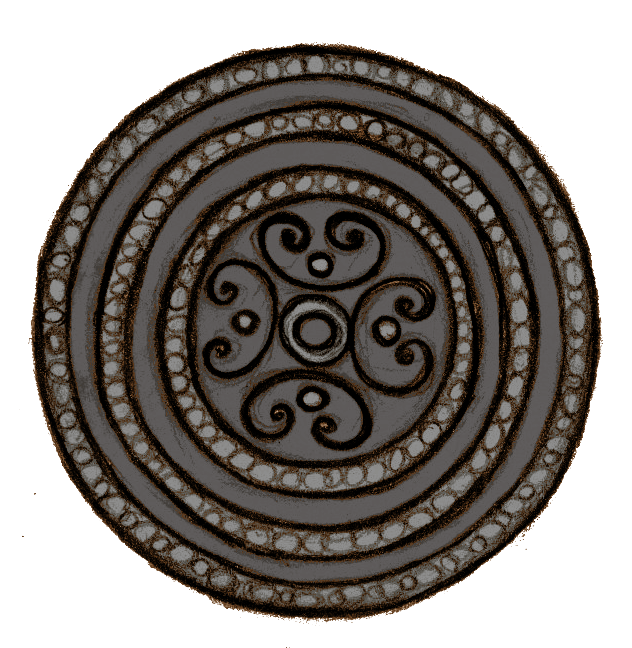
\includegraphics[height=30mm]{img/Jorvik/objects/metal/disk brooch}}\\
		\DIFaddFL{Disk Brooch }& \\ 
		\textbf{\DIFaddFL{Price:}} & \\
		\DIFaddFL{4.41 silver }& \\ 
		\textbf{\DIFaddFL{Description:}} & \\
		\multicolumn{2}{p{12cm}}{Disk Brooches were another popular design of jewellery worn by the Viking men and women. They would be used to fasten clothing like cloaks or to support a chain bearing useful objects or more jewellery. The brooches could be set with precious stones like Amber, if you could afford them.}\\
		\bottomrule
	\end{tabular}
\end{table} \DIFaddend